The performance analysis will be accomplished in multiple segments. To begin with the assessment, we do the analysis in each frame work using different algorithms and different cluster settings. Following that a performance assessment between the frameworks will be conducted to obtain a  proper idea on how these two frameworks can perform in pretty similar situations. To calculate the performance of the algorithms we used \emph{linux verbose} command.

\subsection{performance analysis on Hadoop}
To execute the performance analysis multiple versions of the code has been prepared and run using Hadoop cluster individually on different cluster settings which is discussed on \ref{sec:background}. Linux command \emph{command time --verbose} has been used at the start of Hadoop command to register the time and resource usage. The results for different methods and settings can be found in Figure~\ref{fig:hPerformance}


\begin{figure}[t]
   \centering
   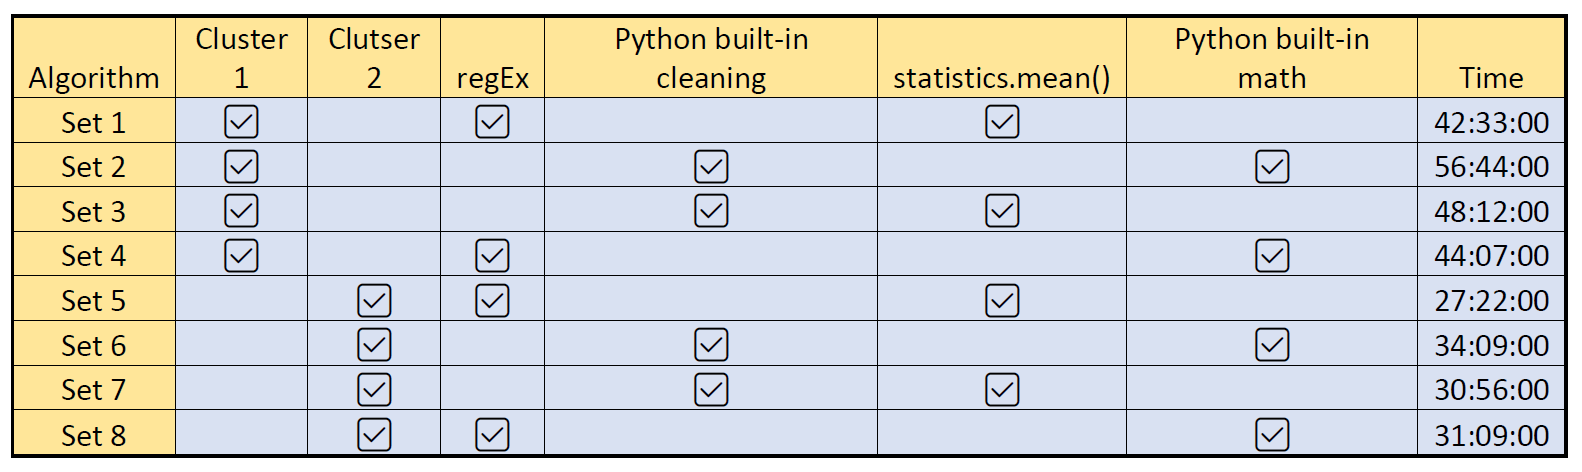
\includegraphics[width=\linewidth]{fig/hPerformance.png}
    \caption{Hadoop Performance statistics}
    \label{fig:hPerformance}
\end{figure}